% CSBP441 Applied Computer Vision -- Final Project Report (CVPR author template)
\documentclass[10pt,twocolumn,letterpaper]{article}
\usepackage{cvpr}              % camera-ready style (names visible)

\usepackage{graphicx}
\usepackage{amsmath,amssymb}
\usepackage{booktabs}
\usepackage{multirow}
\usepackage{xcolor}
\usepackage{tikz}
\usetikzlibrary{arrows.meta,positioning,fit,backgrounds}
\newcommand{\TODO}[1]{\textbf{\color{red}[TODO: #1]}}

\definecolor{cvprblue}{rgb}{0.21,0.49,0.74}
\usepackage[pagebackref,breaklinks,colorlinks,allcolors=cvprblue]{hyperref}
\def\confName{CSBP441}
\def\confYear{2026}

\title{The Road as a Ruler: Training-Free Ground-Plane Scale Correction\\for a Monocular 3D Foundation Model}

\author{Makhmud Kholmuminov \qquad Mohamed Ibrahim Almehrzi\\
Abdalkarim Abumashayekh\qquad Mohammed Hussein\\[2pt]
Department of Computer Science and Software Engineering, UAE University\\
{\small CSBP441 Applied Computer Vision, Fall 2026 \quad Code: \url{https://github.com/makhmudlp/GulfMetric}}}

\begin{document}
\maketitle

% =====================================================================
\begin{abstract}
Monocular 3D foundation models now predict depth in metres from a single photo, but their absolute
scale is often wrong, which matters for robots and vehicles that act on these distances. We study a
training-free fix for a vehicle-mounted camera whose height above the road is known: we fit the road
plane in the model's own 3D prediction with RANSAC, read the camera-to-road distance, and rescale the
prediction so that the camera sits at its true height. Applied to a frozen MoGe-2 model on 900 KITTI
test images, this Geometric Scale Correction (GSC) lowers the mean absolute relative depth error from
0.222 to 0.119 ($-46\%$) and improves 97.4\% of images, at 36\,ms extra per image versus about 400\,ms
for the model itself. Our ablation shows that robust (RANSAC) plane fitting is essential, and that
combining GSC with the true focal length is, surprisingly, worse than GSC alone. GSC fails on streets
lined with parked cars, where the fitted plane is not the road; a simple plausibility check added after
this analysis reduces the error further to 0.097.
\end{abstract}

% =====================================================================
\section{Introduction}
\label{sec:intro}

Knowing \emph{how far} things are is a basic requirement for autonomous driving, mobile robots and
augmented reality. Recent monocular foundation models~\cite{yin2023metric3d,piccinelli2024unidepth,
bochkovskii2025depthpro,wang2025moge2} predict metric depth from a single RGB image and generalise
well across scenes. Their remaining weakness is \emph{absolute scale}: a prediction can have the right
shape yet be uniformly too small or too large, \eg reporting a car at 10\,m that is actually 13\,m
away. A single photo cannot fully disambiguate a small nearby scene from a large distant one.

Many deployed cameras, however, come with free geometric side information: a camera mounted on a car
or robot sits at a known, fixed height above the ground. We ask a simple, practical question:
\emph{can this known height correct the scale of a frozen 3D foundation model, without any training,
and at what cost?}

Our approach, Geometric Scale Correction (GSC), treats the road as a ruler. We fit a plane to the road
in the model's predicted point cloud with RANSAC~\cite{fischler1981ransac}, measure how high the model
believes the camera is, and rescale the whole prediction by the ratio of true to predicted height.
Ground-plane scale recovery itself is a classical idea in monocular odometry~\cite{song2014robust} and
has been used as a training signal~\cite{cecille2024groco}; our contribution is to apply it as a
lightweight post-processing step to a modern foundation model and to measure carefully when it helps.
Concretely, we contribute:
\begin{itemize}
  \item a training-free GSC step for the frozen MoGe-2 model~\cite{wang2025moge2};
  \item a controlled evaluation on 900 KITTI images~\cite{geiger2012kitti,uhrig2017sparsity} that
  separates the effects of focal length, scale correction and robust fitting, together with runtime;
  \item a failure analysis that identifies when the assumption breaks (crowded streets) and a simple
  plausibility check that addresses it.
\end{itemize}

% =====================================================================
\section{Related Work}
\label{sec:related}

\paragraph{Monocular metric depth.}
Early learning-based methods regressed depth with CNNs~\cite{eigen2014depth} and were trained per
dataset. Recent models aim for zero-shot metric depth across cameras. Metric3D~\cite{yin2023metric3d}
and UniDepth~\cite{piccinelli2024unidepth} reason explicitly about camera intrinsics, Depth Anything
V2~\cite{yang2024dav2} and Depth Pro~\cite{bochkovskii2025depthpro} scale up training data, and
MoGe-2~\cite{wang2025moge2} predicts a metric 3D point map with sharp details. These models still
inherit the scale ambiguity of single images, which we target.

\paragraph{Scale from the ground plane.}
Monocular visual odometry recovers metric scale from the known camera height above a detected ground
plane~\cite{song2014robust}. GroCo~\cite{cecille2024groco} uses a ground constraint to train metric
self-supervised depth networks. In contrast, we keep the network frozen and apply the constraint only
at test time, which makes the step model-agnostic and cheap.

% =====================================================================
\section{Method}
\label{sec:method}

\begin{figure*}[t]
\centering
\resizebox{\textwidth}{!}{%
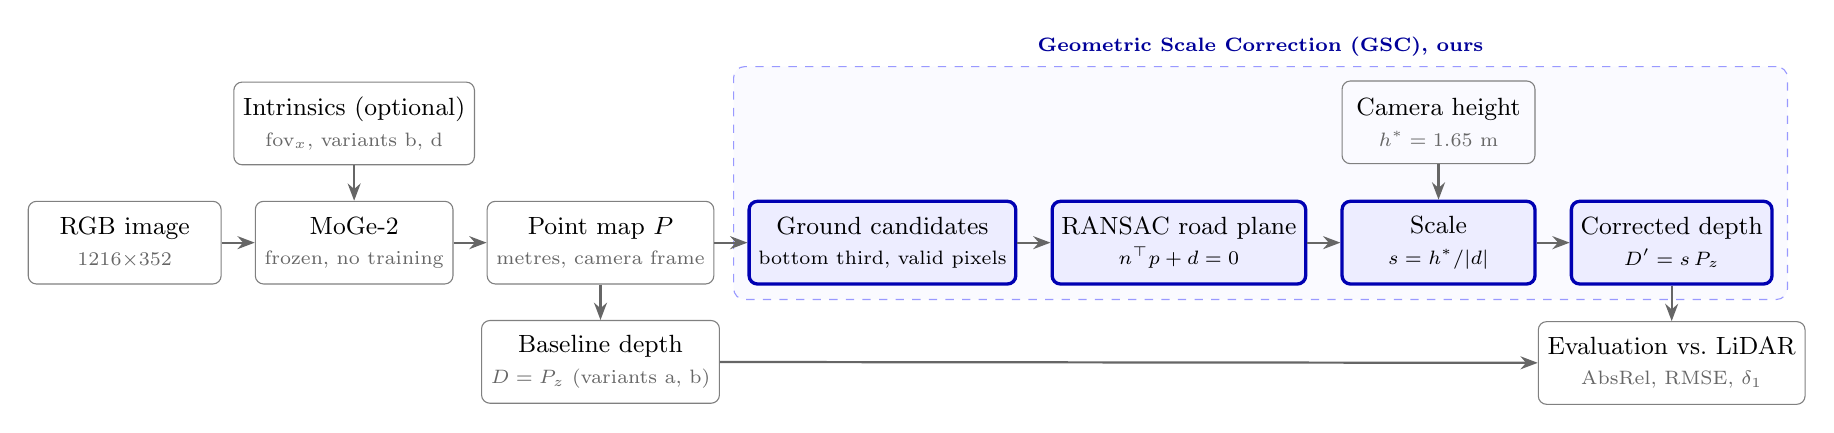
\begin{tikzpicture}[
  box/.style={draw=black!50, rounded corners=3pt, minimum height=1.05cm, minimum width=2.45cm,
              align=center, font=\small},
  ours/.style={box, draw=blue!70!black, very thick, fill=blue!7},
  arr/.style={-{Stealth[length=2.2mm]}, black!60, thick},
  node distance=0.42cm]
  \node[box] (img) {RGB image\\{\scriptsize\color{black!60}$1216{\times}352$}};
  \node[box, right=of img] (moge) {MoGe-2\\{\scriptsize\color{black!60}frozen, no training}};
  \node[box, right=of moge] (pm) {Point map $P$\\{\scriptsize\color{black!60}metres, camera frame}};
  \node[ours, right=of pm] (cand) {Ground candidates\\{\scriptsize bottom third, valid pixels}};
  \node[ours, right=of cand] (ransac) {RANSAC road plane\\{\scriptsize $n^\top p + d = 0$}};
  \node[ours, right=of ransac] (scale) {Scale\\{\scriptsize $s = h^{*}/|d|$}};
  \node[ours, right=of scale] (out) {Corrected depth\\{\scriptsize $D' = s\,P_z$}};
  \node[box, above=0.45cm of moge] (K) {Intrinsics (optional)\\{\scriptsize\color{black!60}$\mathrm{fov}_x$, variants b, d}};
  \node[box, above=0.45cm of scale] (h) {Camera height\\{\scriptsize\color{black!60}$h^{*}=1.65$ m}};
  \node[box, below=0.45cm of pm] (base) {Baseline depth\\{\scriptsize\color{black!60}$D = P_z$ (variants a, b)}};
  \node[box, below=0.45cm of out] (eval) {Evaluation vs.\ LiDAR\\{\scriptsize\color{black!60}AbsRel, RMSE, $\delta_1$}};
  \draw[arr] (img) -- (moge); \draw[arr] (moge) -- (pm); \draw[arr] (pm) -- (cand);
  \draw[arr] (cand) -- (ransac); \draw[arr] (ransac) -- (scale); \draw[arr] (scale) -- (out);
  \draw[arr] (K) -- (moge); \draw[arr] (h) -- (scale); \draw[arr] (pm) -- (base);
  \draw[arr] (out) -- (eval); \draw[arr] (base) -- (eval);
  \begin{scope}[on background layer]
    \node[draw=blue!40, dashed, rounded corners=4pt, fill=blue!2, inner sep=5pt, fit=(cand)(out)(h),
          label={[font=\scriptsize\bfseries, text=blue!60!black]above:Geometric Scale Correction (GSC), ours}] {};
  \end{scope}
\end{tikzpicture}}
\vspace{-1.5em}
\caption{\textbf{Pipeline.} A frozen MoGe-2 model predicts a metric point map. GSC fits the road plane
with RANSAC in the lower image, reads the camera-to-road distance $|d|$, and rescales the prediction so
that the camera sits at its known height $h^{*}$. Baseline and corrected depths are evaluated against
the same LiDAR ground truth.}
\label{fig:pipeline}
\end{figure*}

\paragraph{Baseline.}
Our baseline is MoGe-2~\cite{wang2025moge2} (public ViT-L checkpoint, frozen, fp16 inference). For an
image of width $W$ it returns a point map $P \in \mathbb{R}^{H\times W\times 3}$ in camera coordinates
($x$ right, $y$ down, $z$ forward) and a validity mask; the predicted depth is $D = P_z$. MoGe-2
either estimates the field of view itself (variant a) or accepts a known one, which we compute from
the KITTI intrinsics as $\mathrm{fov}_x = 2\arctan\big(W/(2f_x)\big)$ (variant b).

\paragraph{Geometric Scale Correction.}
We assume that the prediction is correct up to a global factor $s$ (true geometry $\approx sP$) and
that the camera sits at a known height $h^{*}$ above a locally planar road ($h^{*}=1.65$\,m in
KITTI~\cite{geiger2012kitti}). The camera-to-road distance in the \emph{predicted} geometry is then
$h^{*}/s$, so measuring it yields $s$. GSC has three steps (\cref{fig:pipeline}):
(1)~\emph{Ground candidates}: valid 3D points in the bottom third of the image, which for a
forward-facing vehicle camera is dominated by nearby road; at most 20{,}000 are sampled.
(2)~\emph{Robust plane fit}: RANSAC~\cite{fischler1981ransac} with 300 three-point hypotheses
$n^\top p + d = 0$, $\lVert n\rVert=1$. Hypotheses tilted more than ${\approx}37^\circ$ from
horizontal ($|n_y| \le 0.8$) are discarded, a point is an inlier if $|n^\top p + d| < \tau$, and the
best hypothesis is refined by a least-squares (SVD) fit to its inliers.
(3)~\emph{Rescaling}: with a unit normal, $h_{\text{pred}} = |d|$ and
\begin{equation}
  s = h^{*}/h_{\text{pred}}, \qquad P' = s\,P, \qquad D' = s\,D .
  \label{eq:scale}
\end{equation}
If fewer than 500 inliers are found, GSC falls back to $s=1$. It adds no learned parameters; its cost
is dominated by scoring the RANSAC hypotheses.

\paragraph{Plausibility check (post hoc).}
The failure analysis (\cref{sec:failures}) showed that RANSAC can lock onto parked cars instead of
the road, giving implausible factors of $4$--$15\times$. We therefore also report a simple guard, fixed
a priori and not tuned on test data: a correction is accepted only if $0.5 \le s \le 2$, otherwise the
uncorrected prediction is kept. Because it was introduced after inspecting test results, we report it
separately.

\paragraph{Compared variants.}
(a)~MoGe-2 with estimated focal length; (b)~MoGe-2 with true focal length; (c)~(a)\,+\,GSC;
(d)~(b)\,+\,GSC; (d$'$)~as (d) but with a plain least-squares plane over all candidates (no RANSAC);
and an \emph{oracle} that rescales (a) by $\mathrm{median}(D_{\text{gt}})/\mathrm{median}(D)$ using the
ground truth, an upper bound for any global-scale correction.

% =====================================================================
\section{Experimental Setup}
\label{sec:setup}

\paragraph{Dataset and split.}
Our proposal planned a new set of UAE phone photos with laser-measured distances. In direct sunlight
the laser dot was not visible, so the measurements were unreliable, and we moved to a public benchmark.
We use the KITTI depth ``selected validation'' set~\cite{geiger2012kitti,uhrig2017sparsity}: 1000
images ($1216\times352$), each with LiDAR ground-truth depth and camera
intrinsics. File names are sorted alphabetically; the first 100 form a \emph{dev} split, used only to
choose $\tau$, and the remaining 900 (from 11 driving sequences) form the \emph{test} split on which all numbers are
reported.
The split lists are fixed in our repository. KITTI is released under CC BY-NC-SA 3.0.

\paragraph{Metrics.}
Following standard practice~\cite{eigen2014depth}, for each image we use pixels with ground truth in
$(0, 80]$\,m, clip predictions to $[10^{-3}, 80]$\,m, and compute the absolute relative error
$\text{AbsRel} = \frac{1}{N}\sum |D-D_{\text{gt}}|/D_{\text{gt}}$, the RMSE in metres, and
$\delta_1$, the share of pixels with $\max(D/D_{\text{gt}}, D_{\text{gt}}/D) < 1.25$. Scores are
averaged over images. All variants use the same images and pixels.

\paragraph{Threshold selection and implementation.}
On the dev split we swept $\tau \in \{0.03, 0.05, 0.10, 0.20, 0.30\}$\,m for variant (d) and obtained
AbsRel 0.110, 0.105, 0.101, \textbf{0.100}, 0.144, with no fallbacks; we use $\tau = 0.2$\,m. All runs
use Google Colab with one NVIDIA Tesla T4 (15\,GB), PyTorch and NumPy; runtimes are measured after a
warm-up with GPU synchronisation. The full test run (900 images, two model passes each) took about
51\,min.

% =====================================================================
\section{Results}
\label{sec:results}

\begin{table}[t]
\centering
\small
\setlength{\tabcolsep}{3.5pt}
\begin{tabular}{@{}lcccc@{}}
\toprule
Variant & AbsRel$\downarrow$ & RMSE$\downarrow$ & $\delta_1\uparrow$ & vs.\ (a) \\
\midrule
(a) MoGe-2 (baseline)         & 0.222 & 4.62 & 39.6 & -- \\
(b) + true focal length       & 0.133 & 3.86 & 86.0 & $-40\%$ \\
(c) + GSC                     & \textbf{0.119} & \textbf{3.24} & \textbf{92.4} & $\mathbf{-46\%}$ \\
(d) + true focal + GSC        & 0.148 & 4.24 & 82.1 & $-33\%$ \\
(d$'$) (d), LS plane, no RANSAC & 0.413 & 7.70 & 51.0 & $+86\%$ \\
\midrule
\multicolumn{5}{@{}l}{\emph{Added after failure analysis (\cref{sec:failures}):}} \\
(c) + plausibility check      & 0.097 & 2.97 & 92.9 & $-57\%$ \\
(d) + plausibility check      & 0.122 & 3.95 & 82.9 & $-45\%$ \\
\midrule
Oracle median scaling (uses GT) & 0.055 & 2.58 & 97.4 & $-75\%$ \\
\bottomrule
\end{tabular}
\vspace{-0.5em}
\caption{\textbf{Main comparison} on the 900 KITTI test images (RMSE in m, $\delta_1$ in \%). All
rows use the same frozen MoGe-2 model. The oracle uses ground truth and is only an upper bound.}
\label{tab:main}
\end{table}

\begin{figure}[t]
\centering
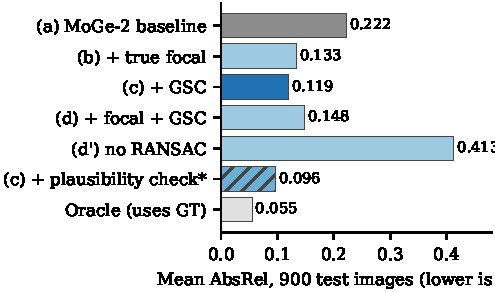
\includegraphics[width=\linewidth]{figures/absrel_bar.pdf}
\vspace{-1.8em}
\caption{Mean AbsRel per variant (lower is better). *Plausibility check added after the failure
analysis.}
\label{fig:bar}
\end{figure}

\paragraph{Main result.}
\Cref{tab:main} and \cref{fig:bar} summarise the comparison. GSC alone (c) lowers the mean AbsRel of
MoGe-2 from 0.222 to 0.119 ($-46\%$) and raises $\delta_1$ from 39.6\% to 92.4\%. The gain is
consistent rather than driven by a few images: (c) is better than the baseline on 97.4\% of test
images, and the median AbsRel drops from 0.222 to 0.085. Our hypothesis was that GSC reduces AbsRel by
at least 30\% while adding under 30\,ms per image. The accuracy part holds for both GSC variants
($-46\%$ and $-33\%$); the runtime part narrowly fails (\cref{tab:cost}), so the hypothesis is
\emph{partly supported}.

\paragraph{Ablation.}
Each component matters. Giving MoGe-2 the true focal length (b) already removes much of the scale
error ($-40\%$), confirming that focal-length errors are a major source of scale errors. Robust fitting
is essential: replacing RANSAC by a least-squares plane (d$'$) makes results \emph{worse} than the
baseline (0.413), because cars and curbs in the lower image pull the plane. Surprisingly, combining
the true focal length with GSC (d) is worse than GSC alone (0.148 vs.\ 0.119; (d) beats (c) on only
28\% of images), although (d) still improves on (b) in 62\% of images. The estimated scale is also
less stable for (d) (5--95\% range of $s$: 0.76--1.30 vs.\ 1.07--1.40 for (c)). We hypothesise that
forcing the field of view makes MoGe-2's ground geometry less self-consistent, but we have not verified
this. The gap to the oracle (0.119 vs.\ 0.055) shows that a global scale fixes only part of the error;
the remainder comes from shape errors that no single factor can correct.

\begin{table}[t]
\centering
\small
\setlength{\tabcolsep}{4pt}
\begin{tabular}{@{}lc@{\hspace{10pt}}lc@{}}
\toprule
\multicolumn{2}{@{}l}{\emph{Cost per image (T4)}} & \multicolumn{2}{l@{}}{\emph{AbsRel by distance, (a)\,$\to$\,(d)}} \\
\midrule
MoGe-2, est.\ focal & 442\,ms & 0--20\,m  & 0.225\,$\to$\,0.139 \\
MoGe-2, true focal  & 379\,ms & 20--40\,m & 0.201\,$\to$\,0.170 \\
GSC mean / median   & 36 / 31\,ms & 40--80\,m & 0.232\,$\to$\,0.206 \\
Peak GPU memory     & 2.38\,GB & GSC fallbacks & 0\% \\
\bottomrule
\end{tabular}
\vspace{-0.5em}
\caption{\textbf{Cost and error by distance.} GSC adds under 10\% to the model's runtime; its gain is
largest at short range, where the road plane is best observed.}
\label{tab:cost}
\end{table}

\paragraph{Cost and distance.}
GSC needs 36\,ms per image on average (median 31\,ms, 95th percentile 64\,ms), under 10\% of the
380--440\,ms that MoGe-2 itself requires, and no extra GPU memory (\cref{tab:cost}). It never fell back
on the test set. Its improvement is largest within 20\,m of the car ($-38\%$) and smaller beyond 40\,m
($-11\%$), consistent with the road being observed only near the vehicle.

\begin{figure*}[t]
\centering
\IfFileExists{figures/qualitative.png}{%
  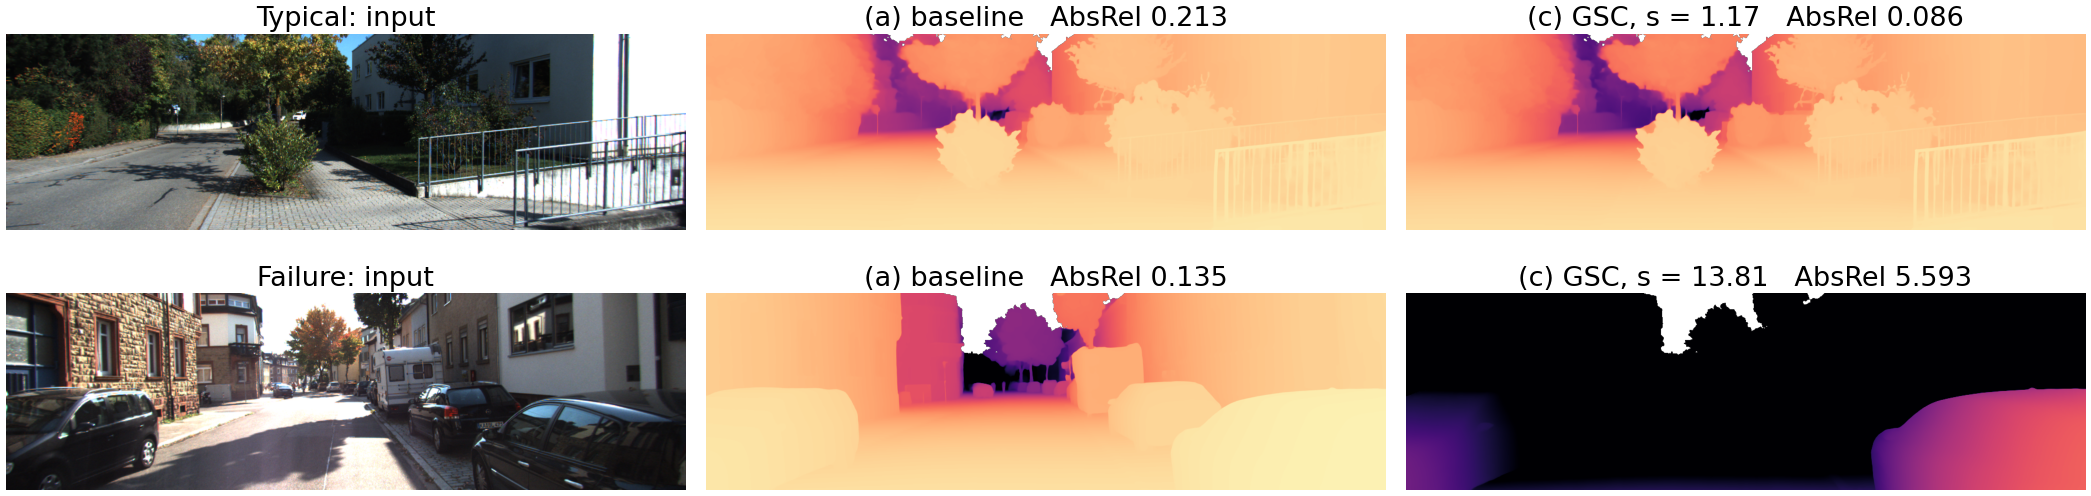
\includegraphics[width=\textwidth]{figures/qualitative.png}}{%
  \fbox{\parbox[c][3.2cm][c]{0.96\textwidth}{\centering\TODO{insert figures/qualitative.png from notebook cell 12}}}}
\vspace{-0.8em}
\caption{\textbf{Qualitative results.} Top: a typical test image (median improvement; AbsRel
0.213\,$\to$\,0.086, $s=1.17$). Bottom: the worst case for (c), a narrow street lined with parked cars
(\texttt{drive\_0095}), where the fitted ``road'' plane lies on the cars and the scale explodes
($s=13.8$, AbsRel 0.135\,$\to$\,5.59). Columns: input, baseline (a) depth, GSC (c) depth; colour
scale 0--80\,m.}
\label{fig:qual}
\end{figure*}

% =====================================================================
\section{Failure Analysis and Limitations}
\label{sec:failures}

GSC fails rarely but badly. Seven test images have AbsRel above 1 for variant (d), and six of them come
from a single sequence, \texttt{drive\_0036}, a street lined with parked cars on both sides; the
remaining one (\cref{fig:qual}, bottom) is a similar narrow street. There, the lower image is dominated
by car bodies; RANSAC finds a
near-horizontal plane on the cars, the model appears to sit only 0.11--0.41\,m above this ``road'',
and the scale explodes to $4$--$15\times$ (oracle scale $\approx1.2$). As a result, (d) is worse than
the baseline on this sequence on average (AbsRel 0.266 vs.\ 0.226), while it helps strongly elsewhere
(\eg 0.274\,$\to$\,0.113 on \texttt{drive\_0047}).

Because a metric model is unlikely to be off by more than a factor of two, we added the plausibility
check of \cref{sec:method} after this analysis. It rejects only 7--8 of 900 corrections and lowers the
mean AbsRel to 0.097 for (c) and 0.122 for (d) (\cref{tab:main}). The outcome is insensitive to the
exact bounds: $[0.33, 3]$ and $[0.67, 1.5]$ give 0.097 for (c). Since the rule was chosen after seeing
these failures, it should be confirmed on new data.

\paragraph{Limitations.}
GSC requires a known camera height and a visible, roughly planar road near the camera, so slopes, hills,
crowded scenes and handheld cameras violate its assumptions. All results come from one benchmark with a
single camera rig in one city, and we did not tune the ground region or test other foundation models.
Our planned evaluation on UAE scenes (glass facades, sand) remains future work and would require a
reliable way to measure ground truth outdoors.

% =====================================================================
\section{Conclusion}
\label{sec:conclusion}

A known camera height turns the road into a ruler: without any training, fitting the road plane in a
frozen MoGe-2 prediction and rescaling it nearly halves the depth error on KITTI and improves almost
every image, at under 10\% extra runtime. Robust fitting is essential, adding the true focal length on
top did not help, and crowded streets are the main failure mode, which a simple plausibility check
largely contains.

% =====================================================================
\section*{Implementation, Attribution and Contributions}
\label{sec:attribution}
\textbf{Built by the team:} the GSC step (ground selection, constrained RANSAC, rescaling, fallback),
the plausibility check, the evaluation pipeline (split, metrics, ablation, timing) and all experiments
and analyses. \textbf{External resources:} MoGe-2 code and pretrained weights~\cite{wang2025moge2};
the KITTI depth benchmark~\cite{geiger2012kitti,uhrig2017sparsity}; PyTorch, NumPy, OpenCV, pandas and
Matplotlib; Google Colab. \textbf{Generative AI:} an AI assistant (Claude, Anthropic) was used to help
write code and draft this report; the team ran all experiments, checked every reported number against
the result files, and is responsible for the content. \textbf{Contributions:} All four members contributed to the project idea, the proposal, the
choice of KITTI and the method design, and reviewed the final report.
Makhmud: GSC implementation, pipeline code and experiments, report writing.
Mohamed Ibrahim Almehrzi: related-work survey, presentation slides and demo.
Abdalkarim Abumashayekh: dataset setup and reproduction instructions, README, reference verification.
Mohammed Hussein: verification of all reported numbers against the result files, figure review,
proofreading.

{
    \small
    \bibliographystyle{ieeenat_fullname}
    \bibliography{refs}
}

\end{document}
